\documentclass[11pt]{article}
\usepackage{fullpage,amsmath,amsfonts,mathpazo,microtype,nicefrac,graphicx,verbatimbox,listings,hyperref,enumitem,amssymb,float,fancyhdr,caption,subcaption}
\DeclareGraphicsExtensions{.pdf,.eps,.png}

% Margins
% \topmargin=-0.45in
% \evensidemargin=0in
% \oddsidemargin=0in
% \textwidth=6.5in
% \textheight=9.0in
% \headsep=0.25in

% \linespread{1.1} % Line spacing

% % Set up the header and footer
% \pagestyle{fancy}
% \lhead{\hmwkAuthorName} % Top left header
% \chead{\hmwkClass\ (\hmwkClassInstructor\ \hmwkClassTime): \hmwkTitle} % Top center header
% \rhead{\firstxmark} % Top right header
% \lfoot{\lastxmark} % Bottom left footer
% \cfoot{} % Bottom center footer
% \rfoot{Page\ \thepage\ of\ \pageref{LastPage}} % Bottom right footer
% \renewcommand\headrulewidth{0.4pt} % Size of the header rule
% \renewcommand\footrulewidth{0.4pt} % Size of the footer rule

% \setlength\parindent{0pt} % Removes all indentation from paragraphs

%----------------------------------------------------------------------------------------
%   TITLE PAGE
%----------------------------------------------------------------------------------------

\title{
\vspace{1cm}
\textmd{\textbf{AC209a Data Science Project: Data Science with User Ratings and Reviews}}\\
% \normalsize\vspace{0.1in}\small{Due\ on\ \hmwkDueDate}\\
% \vspace{0.1in}\large{\textit{\hmwkClassInstructor\ \hmwkClassTime}}
}

\author{\textbf{Andrew Ross, Sophie Hilgard, Reiko Nishihara, Nick Hoernle}}
\date{\today} % Insert date here if you want it to appear below your name

%----------------------------------------------------------------------------------------

\begin{document}

\maketitle

\section*{Data Source}
We downloaded the data from the `Yelp Dataset Challenge' (\url{https://www.yelp.com/dataset_challenge}). The data contains in total 2.7M reviews from 687K users for 86K businesses. Business data consist of 15 features including ID, category of business (e.g., fast food, restaurant, nightlife, etc.), city, full address, operation hours, latitude, longitude, review count, and stars earned. User data consist of 11 features including average stars, compliments, elite, number of fans, IDs of his/her friends, name, review count, vote categories, and the month start a yelp review.

\section*{Data Exploration}

\subsection*{Overview Exploration}

\par A simple inspection of the businesses data shows that usful information such as the business categories, latitude and longitude and the average ratings given to a business are all easily available. Similarily, for each user we have information about the number of reviews that they have given, the average rating that they give and the date that they have been `yelping' since.

\begin{figure}[H]
\centering
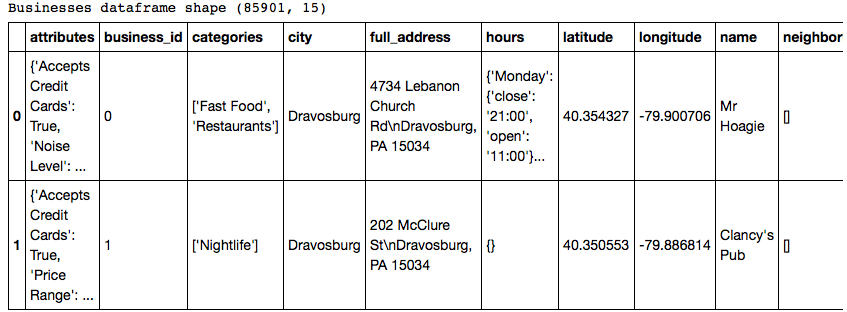
\includegraphics[width=0.7\textwidth]{./ac209/bizdataframe.png}
\caption{Head of Businesses Dataframe}
\end{figure}

\begin{figure}[H]
\centering
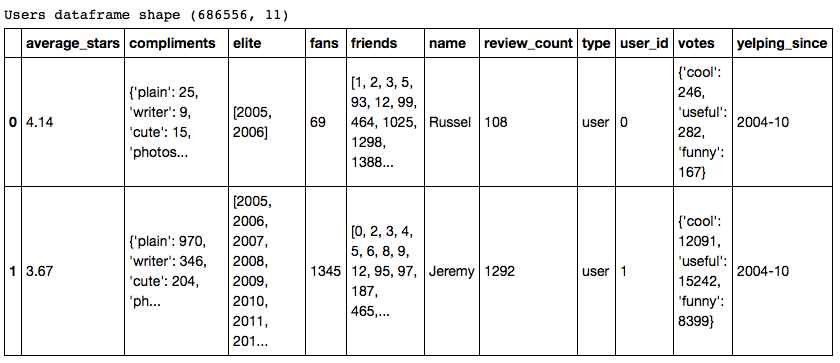
\includegraphics[width=0.7\textwidth]{./ac209/userdataframe.png}
\caption{Head of Users Dataframe}
\end{figure}

A simple summary description of these dataframes is then presented below:

\begin{figure}[H]
\centering
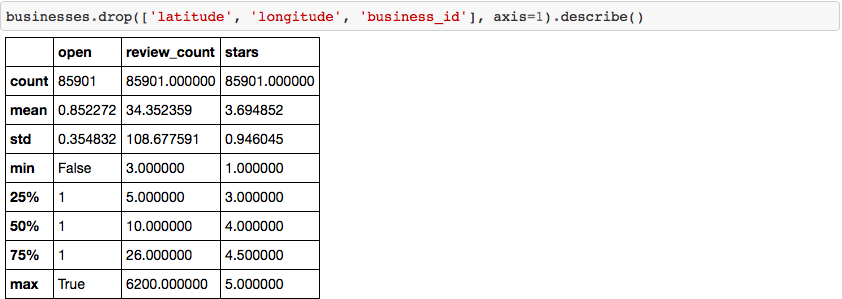
\includegraphics[width=0.9\textwidth]{./ac209/bizdescribe.png}
\caption{Summary statistics of the Businesses Dataframe}
\end{figure}

\begin{figure}[H]
\centering
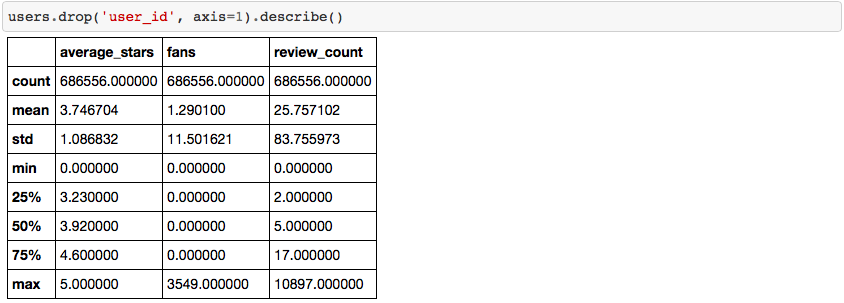
\includegraphics[width=0.9\textwidth]{./ac209/userdescribe.png}
\caption{Summary statistics of the User's Dataframe}
\end{figure}

\par We see from the summary data that most reviewers do not have fans and wrote a small number of reviews. Concretely, the median number of reviews given by a user is 5 yet the mean is 25. This suggests drastically right skewed data (which is intuitive as there is a lower bound of 0 on the number of reviews that a user can give). The inter-quartile range, IQR, for user rating was 3.2 - 4.6, again suggesting that most users rate businesses higher than the midpoint rating of 2.5. Similarly, we see that the businesses receive a mean rating of 3.69, with a mean count of 34.35. The IQR for review count for businesses is 5 to 26, again suggesting that a majority of businesses have a small number of reviews. \\

\par The review counts (number of reviews given by a user and number of reviews received by a business) are dramatically right skewed. We thus, omit the outliers in the below plot to understand the distribution of the $10^{th}$ to $90^{th}$ percentiles for review counts. We still see a hugely right skewed dataset, again intuitively it is more common for many users to rate a few number of businesses and it is more common for many businesses to receive a low number of reviews.

\begin{figure}[H]
\centering
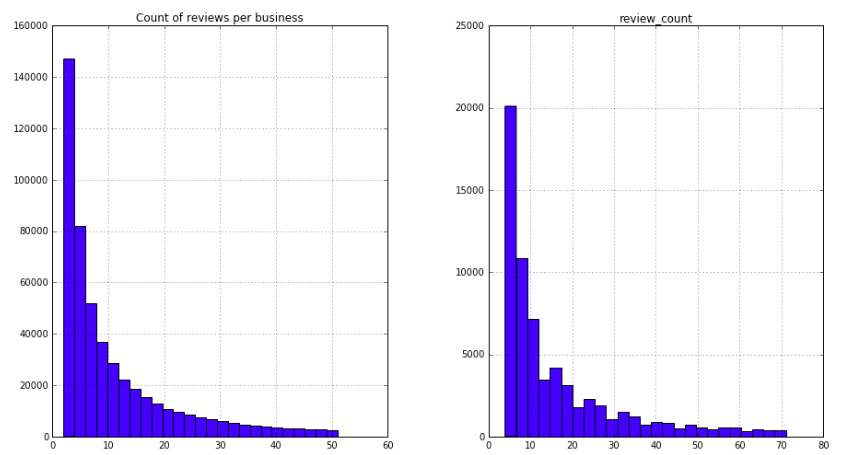
\includegraphics[width=0.9\textwidth]{./ac209/countreviewshist.png}
\caption{Exponentially distributed count of reviews received per business (left) and count of reviews given per user (right)}
\end{figure}

% \par Figures for the count of reviews per user and count of reviews per business show a unimodal distribution with fatter tail in the right side. Most reviewers tend to write a small number of reviews, and therefore most businesses got a small number of reviews. A question that arises from this plot: for the businesses that receive a high number of ratings, are the ratings more or less positive than the businesses that receive a low number of ratings? The same question can be asked of the users.

\subsection*{Time based Exploration}
It was interesting to understand the distribution of the numbers of reviews over time for the yelp data.

\begin{figure}[H]
\centering
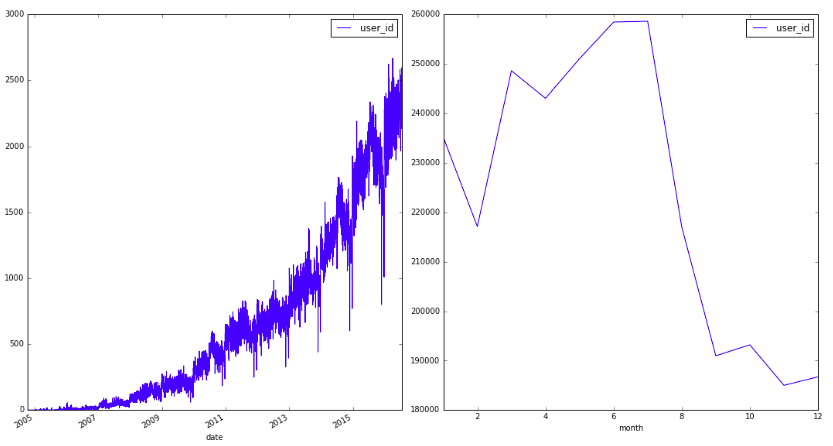
\includegraphics[width=0.9\textwidth]{./ac209/timeseries.png}
\caption{Number of reviews per day on yelp over time}
\end{figure}

We see that the number of reviews that are submitted on the Yelp platform over time is increasing dramatically from when Yelp opened in 2004 to present, were approximately 2500 reviews are submitted per day. Analyzing the number of reviews that are submitted over the course of a year shows that June and July are popular months while November and December show a relevantly lower number of reviews. An interesting point for further exploration is if the business type shows different `high' and `low' seasons and if the popularity of a business or a category of businesses can be tracked over time.

\subsection*{Location based Exploration}

We see that we are given 10 cities from the yelp data. From the metatdata about this database we know that these correspond to (the corresponding number of businesses was calculated for each city):
\begin{itemize}
	\item U.K.: Edinburgh (3480)
	\item Germany: Karlsruhe (1074)
	\item Canada:
		\begin{itemize}
			\item Montreal (5592)
			\item Waterloo (530)
		\end{itemize}
	\item U.S.:
		\begin{itemize}
			\item Pittsburgh (4088)
			\item Charlotte (7160)
			\item Urbana-Champaign (807)
			\item Phoenix (36505)
			\item Las Vegas (23598)
			\item Madison (3067)
		\end{itemize}
\end{itemize}

For the locations part of this study we will therefore narrow the focus to Las Vegas and Phoenix due to the large number of businesses in these cities and the expected restaurant culture that is a perception that is given of these cities.\\

\par For Phoenix the various categories were extracted from the data and the top business categories (by count) are shown below:
\begin{itemize}
	\item `Restaurants', 9428)
	\item `Shopping', 5424
	\item `Food', 3637
	\item `Beauty \& Spas', 3603
	\item `Home Services', 3466
	\item `Health \& Medical', 3420
	\item `Automotive', 2629
	\item `Local Services', 2119
	\item `Nightlife', 1599
	\item `Active Life', 1551
\end{itemize}

We explored any trends in these categories and plotted the data by location. We also color coded the businesses by their average rating (with brown being the highest rating of 5 and gray being the lowest rating of 1). Restaurants are evenly distributed throughout Phoenix with an overwhelming number of highly rated businesses. The other business types are more evenly spread out but the Nightlife category shows a clear `hub' in the city center. Unfortunately, we see no clear areas that are high rated vs low rated areas. This is a specific point of interest (i.e. do certain areas come into and out of popularity) and thus will be investigated further throughout the course of this project.

\begin{figure}[H]
\centering
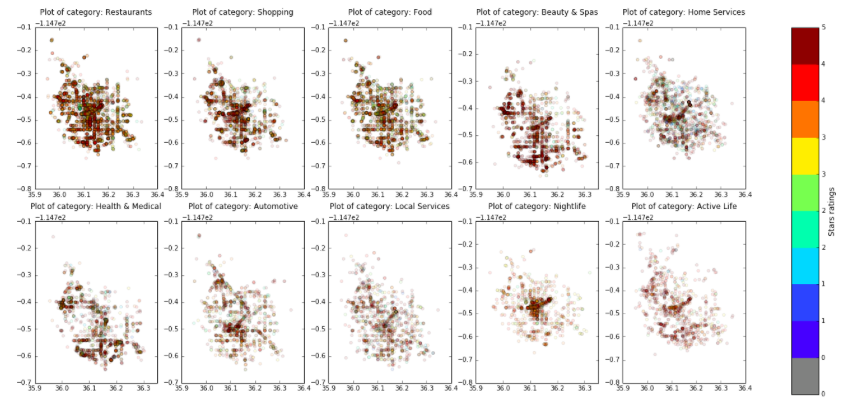
\includegraphics[width=1.1\textwidth]{./ac209/phxstarsbycategorylocation.png}
\caption{Chart showing the top 10 most popular business category plotted by location and colour coded by average review}
\end{figure}

\subsection*{Ratings based Exploration}

We next explored the top rated businesses by introducing a prior model to the rating. We introduced a prior that most businesses will by rated at 2.5 and this has the effect of normalizing the distribution such that the higher rated businesses are required to have a large number of high ratings and similarly, the lower rated businesses are required to have a low number of ratings. The resulting distribution is shown below:
\begin{figure}[H]
\centering
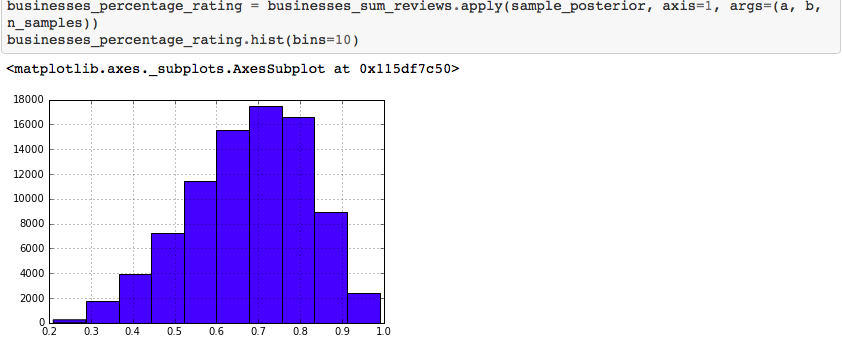
\includegraphics[width=0.9\textwidth]{./ac209/businessespctrating.png}
\caption{Chart showing the top biased businesses}
\end{figure}

Examples from the highest and lowest ranked businesses:
\begin{table}[H]
\centering
\caption{Examples of low and highly ranked businesses}
\label{my-label}
\begin{tabular}{|l||r|}
	\hline
	\textbf{Lowest Ranked Businesses}  & \textbf{Lowest Ranked Businesses} \\ \hline
	A Victory Inn 		 				& Blue Chip Auto Glass \\ \hline
  OnTrac&                        Lockaid USA \\ \hline
  Monitronics Security&                      Stell Roofing \\ \hline
  Anjile Cleaning Service LLC&              Simply Skin Las Vegas \\ \hline
  Website Backup& Khina Eyebrow Threading \& Henna Art \\ \hline
\end{tabular}
\end{table}

\begin{figure}[H]
\centering
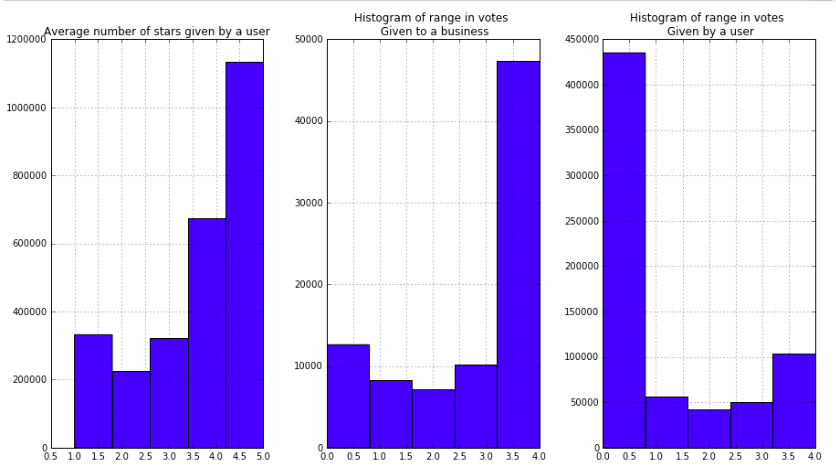
\includegraphics[width=0.9\textwidth]{./ac209/avgstarsusersbusinesses.png}
\caption{Plot of the average and range of ratings that a user gives and the range of ratings that a business receives.}
\end{figure}

\par We see that users typically rate businesses highly (with a clear mode being 5 stars). However, we also note that businesses have a high range of votes (a mode of 4 indicates that users differ in their opinions). The figure also shows that users did not change their rating schema based on the business, and the majority of users rate all businesses within 1 point of each other.


\begin{figure}[H]
\centering
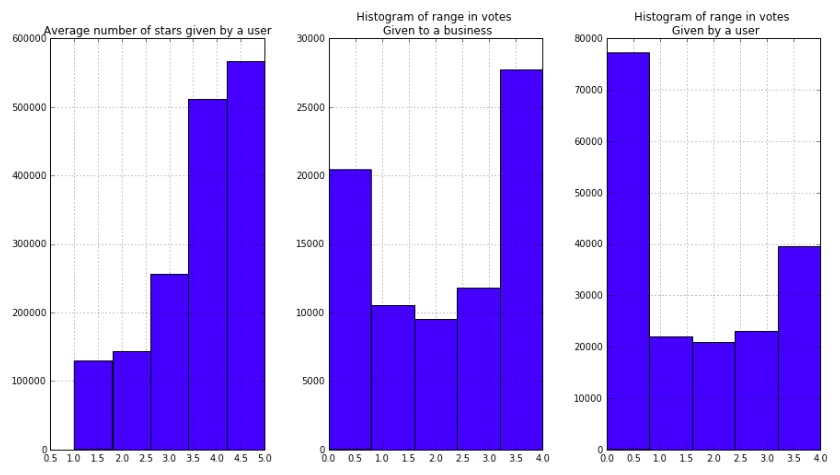
\includegraphics[width=0.9\textwidth]{./ac209/avgstarsusersbusinesses-filter.png}
\caption{}
\end{figure}




\begin{figure}[H]
\centering
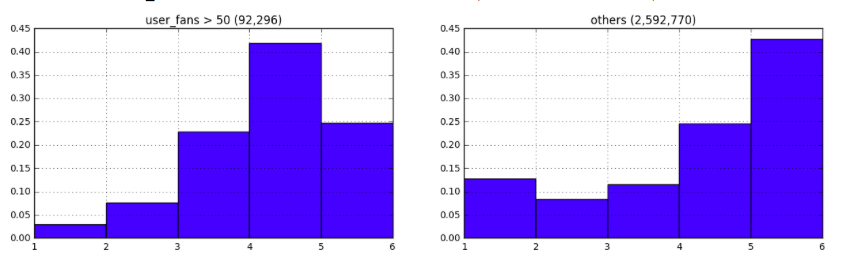
\includegraphics[width=0.9\textwidth]{./ac209/lotsoffans.png}
\end{figure}

\begin{figure}[H]
\centering
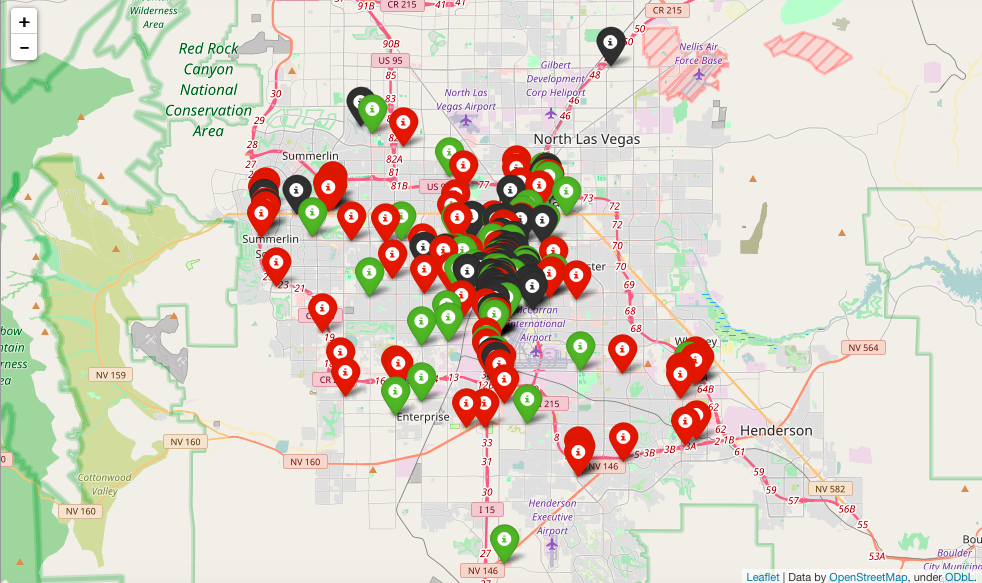
\includegraphics[width=0.9\textwidth]{./ac209/mostreviewsbylocationlv.png}
\end{figure}


\begin{figure}[H]
\centering
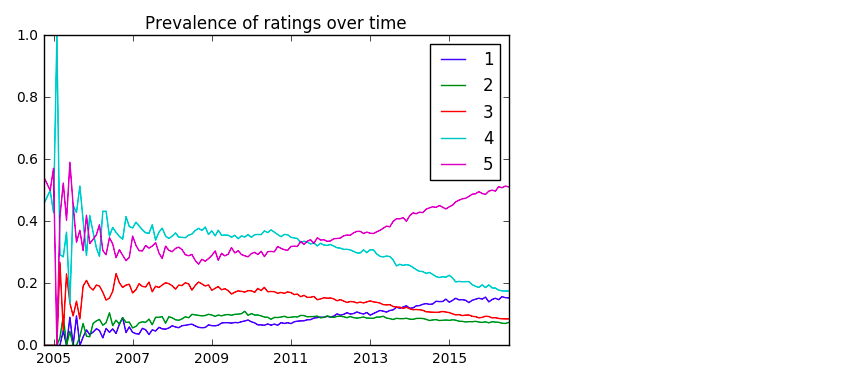
\includegraphics[width=0.9\textwidth]{./ac209/prevalenceofratingsovertime.png}
\end{figure}

\begin{figure}[H]
\centering
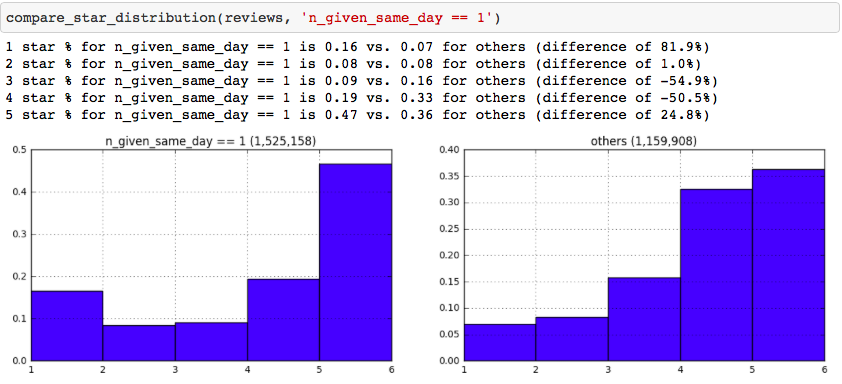
\includegraphics[width=0.9\textwidth]{./ac209/numstarsreviewsperday.png}
\end{figure}

\begin{figure}[H]
\centering
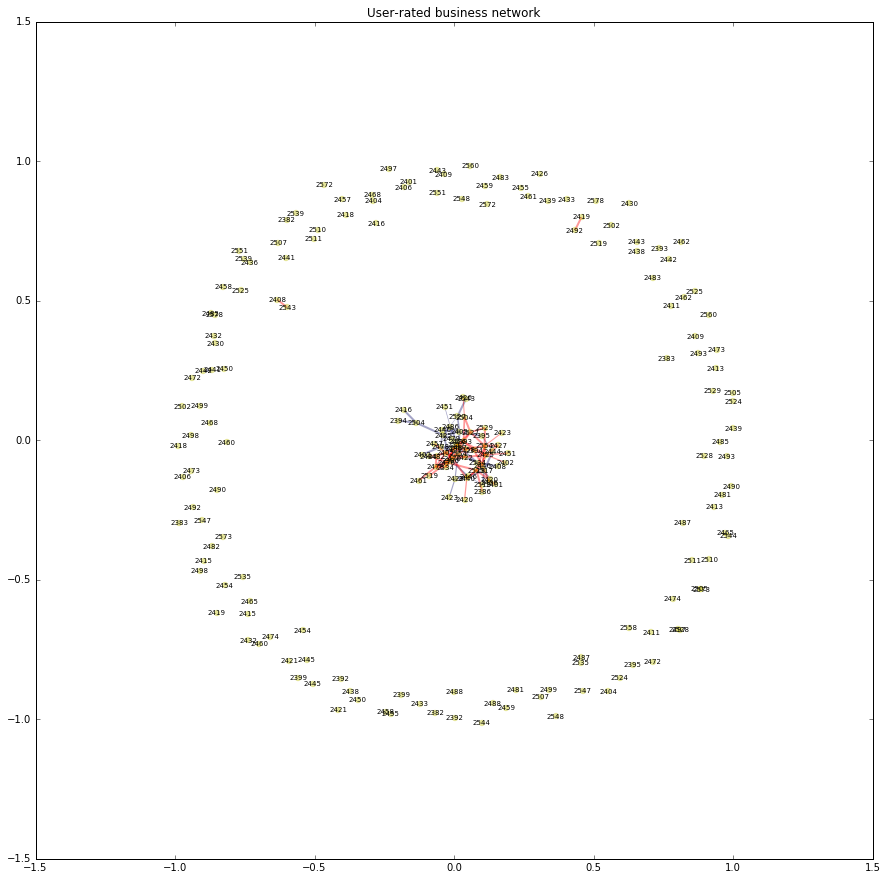
\includegraphics[width=0.9\textwidth]{./ac209/networkanalysis.png}
\end{figure}


\par Now, we plotted average numbers of stars by the number of reviews of users according to the number of reviews in a business. Figures show a modest trend of having higher stars when a business was reviewed by many people. However, we don't see clear relationship among the number of reviews given by a user (or to a business) and the average rating that the business has (or user gives). We can further corroborate this result by analysing the standard deviation in the reviews that a business receives (and a user gives).

\par Using a prior that assumes businesses will not be enjoyed (we wish to overcompensate for the average high ratings of users), we are able to build a more comprehensive likelyhood and thus filter the review somewhat into a more confident top and bottom grouping. The ratings alone are unreliable and we rather wish to include the number of times a business has been rated in a particular manner to calculate the likelihood that this is a favorable (or not) business). For example, if a business is rated poorly twice, this is an unreliable statistic and we do not wish to penalise the business from a median likelihood too dramatically. On the contrary, if a business is rated poorly 100 times, we are confident that users rate the business poorly and we wish to have a low likelihood for enjoyment. In the figure, we show a distribution that corresponds to a probability that this is a good business (i.e., users will like it). On the low end of the scale we have a small number of very poor businesses. We note that these businesses will have a large number of poor ratings. Similarly, on the high end, we see that there is a relatively small number of highly rated businesses. These businesses require a high number of very positive ratings to be rated into this category. We note that we used a fairly aggressive prior assumption that all businesses have a median probability for being liked that is less than 2.5. This is to overcompensate for the generally high ratings. We now have a more normally distributed dataset.



\par In earlier years (i.e., before 2008), the average stars varied very widely from 1 to 5 stars. In contrast, after 2009 onward, the average stars converged to around 4. This is mainly because we have more reviews over time and the mean value became less variable. The rating did not differ according to the month reviewed.

\par When we analyzed the number of repeated reviews by a user, we found that majority of reviews reviewed once.

\end{document}

